\chapter{绪论}

\section{引言}
子痫前期(preeclampsia, PE)又作先兆子痫,是孕妇妊娠期特有的一种多系统进展性疾病, 与妊娠期高血压(gestational hypertension)、子痫(eclampsia)、
慢性高血压并发子痫前期(chronic hypertension with superimposed preeclampsia)以及妊娠合并慢性高血压(chronic hypertension)统称妊娠期
高血压疾病(hypertension disorders of pregnancy, HDP)\cite{OAG9,HDASOM,2000s1}。
原发性高血压与蛋白尿是临床PE患者最有代表性的并发症之一。
随着近年对PE相关研究的深入,世界卫生组织进一步地拓展了PE的涵盖范围,将其定义为:在妊娠20周后出现新发(原发)高血压,在两次间隔4 h或4 h以上的血压(blood pressure, BP)测定中,收缩压(systolic blood pressure, SBP) ≥ 140 mmHg和(或)
舒张压(diastolic blood pressure, DBP) ≥ 90 mmHg,且伴有下列任一项或多项\cite{OAG9,FIGO}:

1、孕妇出现蛋白尿症状,其24 h尿蛋白总量 ≥ 300 mg,或尿蛋白/肌酸酐比值 ≥ 30 mg/mol,或随机尿蛋白检验呈阳性;

2、孕妇无尿蛋白相关症状但伴有以下任一器官或系统功能紊乱、受累受损:心、肺(肺水肿)、肝(血清转氨酶水平为正常值2倍以上)、肾(血肌酐 ≥ 1.1 mg/dl
或为正常值2倍以上)等重要器官功能紊乱,或血液系统(血小板 < 100$\times 10^{9}$/L等)、消化系统、神经系统的异常改变等;

3、胎盘或胎儿生长受限,脐动脉多普勒分析检测异常,甚至出现死胎等症状。

妊娠期高血压疾病可引起严重的母胎并发症,是孕产妇和围产儿病死率升高的主要原因之一\cite{OAG9}。
据世界卫生组织统计,PE在孕妇中发病率高达5\%$ \sim $10\%,是体内大出血以外致使孕妇死亡的第二大危险因素,每年可导致全球范围内约7.6万名孕妇死亡,并进一步导致约50万
名胎儿/婴儿的死亡\cite{DAM2015,LCT2006}。为推广普及人们对PE的认知,同时教育女性了解她们当前及长期的健康风险,
全球孕妇保健组织自2017年起将每年的5月22日确定为世界子痫日(world preeclampsia day)。

就现阶段我国国情而言,排名世界第一的人口基数导致了我国庞大的妊娠孕妇数及新生儿数\cite{nbs2022}。
2022年,浙江省人口普查信息显示,妇女峰值生育率微幅下降、生育高峰年龄区间后移并缩短;妇女晚育现象比较普遍;自全面开放二孩政策后,二孩、多孩生育率持续回升\cite{zjtjj2022}。而临床研究已经证实,
孕妇高龄与多次妊娠均属于可能导致PE的风险因子(risk factors),会增加其PE患病可能\cite{Duckitt2005,FIGO,Yogev2010,Poon2010,Lee2000,Coonrod1995,Robillard1993}。
因此,实现PE的早期预测与快速有效的医学诊断乃至精确治疗与干预,可以有效保障孕妇及围产儿的生命健康安全,具有重大的临床应用价值。
\section{子痫前期发病机制}
截止目前,医学界对PE的病因与发病机制尚无统一的结论,相关研究还在继续进行之中。但得到公认的一点是,PE病发具有异质性,多种因素、机制与通路均对PE的病发有所影响,不能仅以“一元论”的观点对待。
本节对目前多种可能的PE的病因及发病机制进行介绍。

\subsection{主流学说}
目前最为普遍接受的主流学说认为,PE的发病与妊娠早期胎盘功能紊乱密切相关,其病发由子宫螺旋小动脉重铸不足导致\cite{OAG9,Duvekot2010,Ix2009}。子宫螺旋小动脉重铸不足导致PE病发的作用机制可以概括为两个阶段,如\autoref{fig:ppp}所示。
在第一阶段,孕妇子宫螺旋动脉重构受损、出现重铸障碍,绒毛外滋养细胞浸润能力受损,导致胎盘缺血、缺氧,释放多种胎盘因子,该阶段无明显临床现象。在第二阶段,各种胎盘因子进入母体血液循环,导致血管阻力增大,胎盘灌注减少,
促进系统性炎症反应的激活及血管内皮损伤引起PE多样化的临床表现。
\begin{figure}[htbp]
    \centering
    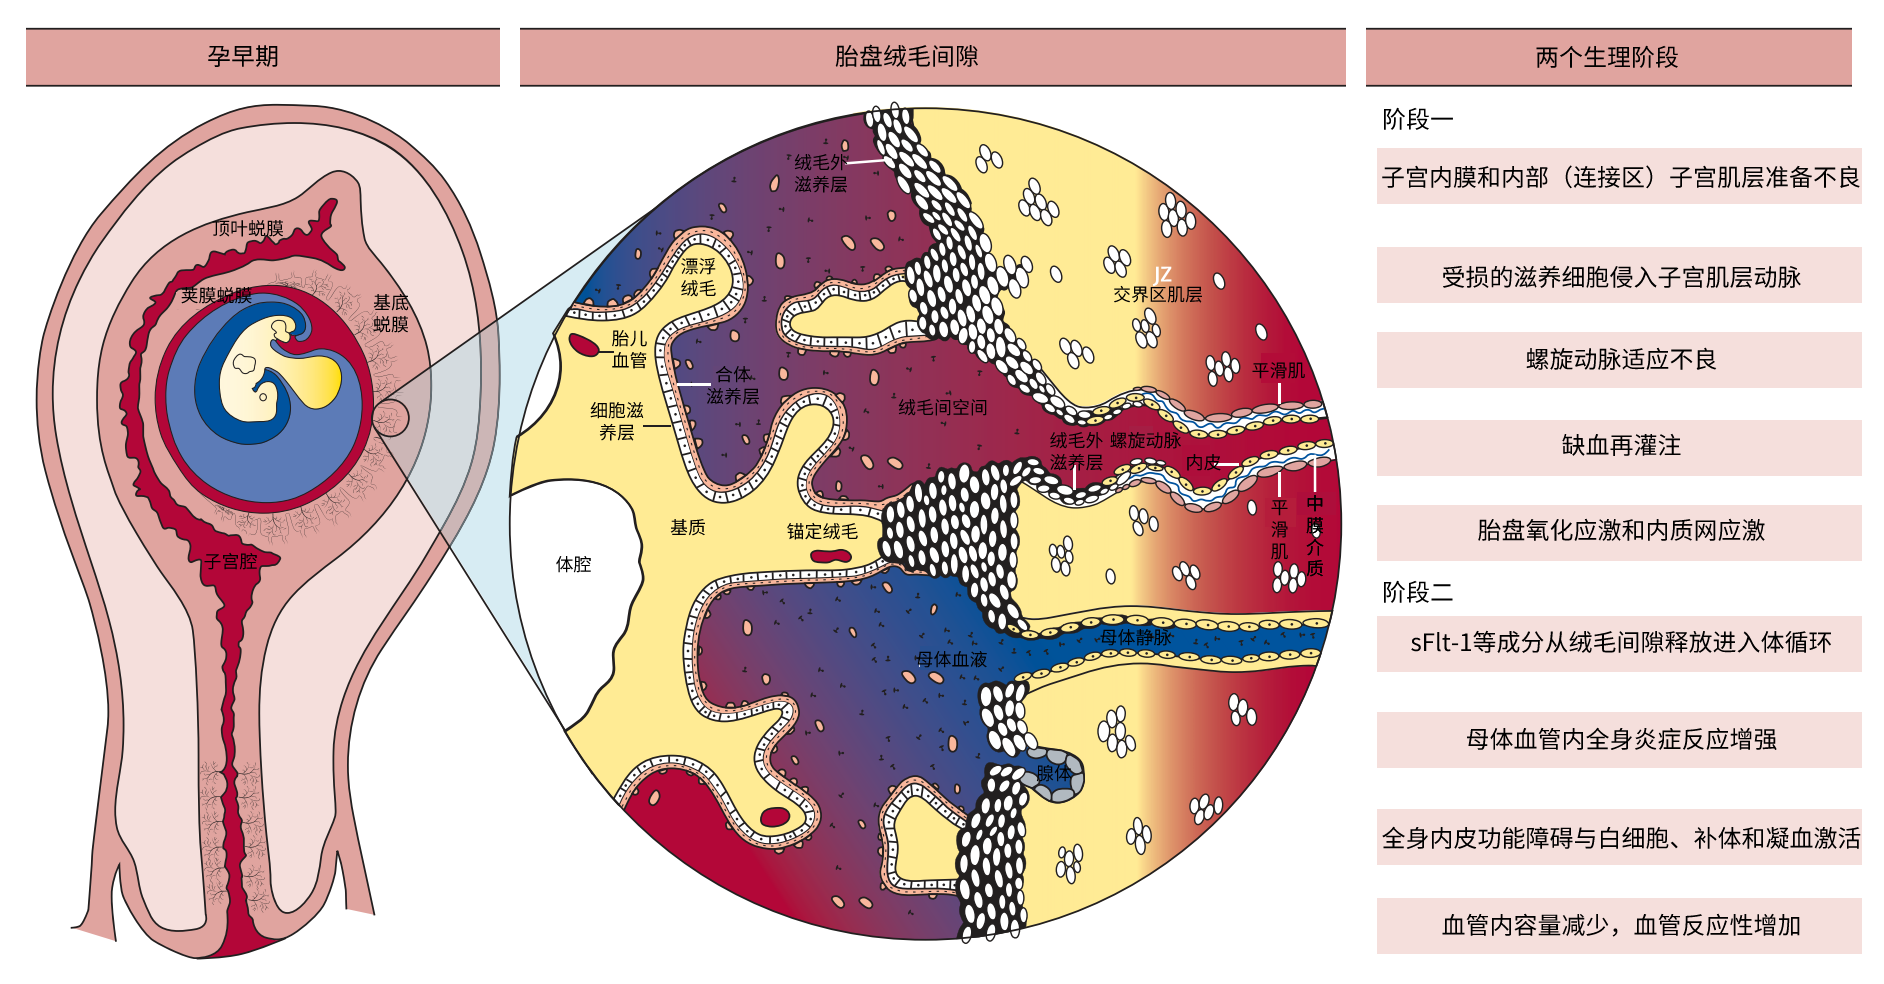
\includegraphics[width=\linewidth]{intro/ppp}
    \caption[子宫螺旋小动脉重铸不足致使PE病发学说示意图]{\label{fig:ppp}子宫螺旋小动脉重铸不足致使PE病发学说示意图\cite{Duvekot2010,Ix2009}}
\end{figure}

\subsection{其他学说}
临床的专家学者们还提出了多种可能的其他PE病发机制,包括炎症免疫过度激活学说、血管内皮细胞损伤及前列腺素合成失调学说、遗传学说、胎盘因子学说及营养不足学说等。

炎症免疫过度激活学说认为PE是母系-父系免疫适应不良导致的,即胎儿胎盘具有的半抗原性移植体特性导致同种异体移植排斥,最终引起的母系同种免疫反应从而诱发PE\cite{Sibai2005,OAG9,Shi2006,Moffett2002}。
血管内皮细胞损伤及前列腺素合成失调观点认为,血管内皮细胞出现损伤后导致前列腺素合成失调,并进一步使扩张血管的物质(如一氧化氮、前列环素等)合成减少,同时使收缩血管的物质(如内皮素、
血栓素等)合成增加,从而促发血管痉挛导致PE病发\cite{OAG9,Sibai2005}。遗传学说则是以PE具有家族倾向性的临床现象为基础\cite{OAG9,Sibai2005,Ge2013}。
而近年来,学者们相继提出的胎盘因子学说\cite{Shi2006}与营养不足学说\cite{OAG9}等假设仍需进一步临床研究与理论研究来证实。
\raggedbottom

\section{子痫前期识别诊断的研究现状}
现代医学对PE的认知经历了漫长的探索\cite{BJOG2016}。早在古希腊Hippocrates时代(约公元前460-370年),医学界就对子痫的症状有一定的认识。但直至18世纪,医学界才将子痫与癫痫加以区分对待。
19世纪中叶,医学界开始认识到子痫之前存在一个前驱状态。法国医生Pierre Rayer首次描述了子痫病发孕妇的蛋白尿症状,英国医生John Lever更进一步证实了蛋白尿与子痫病发的特异性关系。
20世纪初,尿液分析与血压测量开始用于子痫的诊断,同时进一步细化的PE的相关概念开始出现。20世纪中后叶,由于医学诊断技术的发展,多种新的检测指标与技术不断被引入子痫及PE的识别诊断中。
进入21世纪后,由于智能化技术的发展与电子设备的普及,基于医学大数据的人工智能相关研究又成为了新的热点。

本小节将从现阶段临床对PE病发评估的常用检测参数指标、医用检测设备及新兴人工智能检测技术等三方面对PE的识别诊断现状进行介绍。

\subsection{常用检测参数指标}
现阶段临床使用的PE检测参数指标可概括为风险因子(risk factors)与生物标志物(biomarkers)等两大类。

一、风险因子筛查

此前学者的研究表明,孕妇自身的一些基础信息与PE的病发密切相关,这些信息被统称为PE风险因子\cite{Magee2008,FIGO,Lowe2015,Heazell2010}。临床医生往往会以量表问卷的形式向孕妇采集风险因子信息,
对孕妇PE的病发可能进行初筛\cite{risks},如\autoref{fig:risk}所示。常见的PE风险因子及其可能的影响如\autoref{tab:riskfactors}所示。
其中,体重指数(body mass index,BMI)常用作评估人体体重是否位于合理区间。
\begin{figure}[htbp]
    \centering
    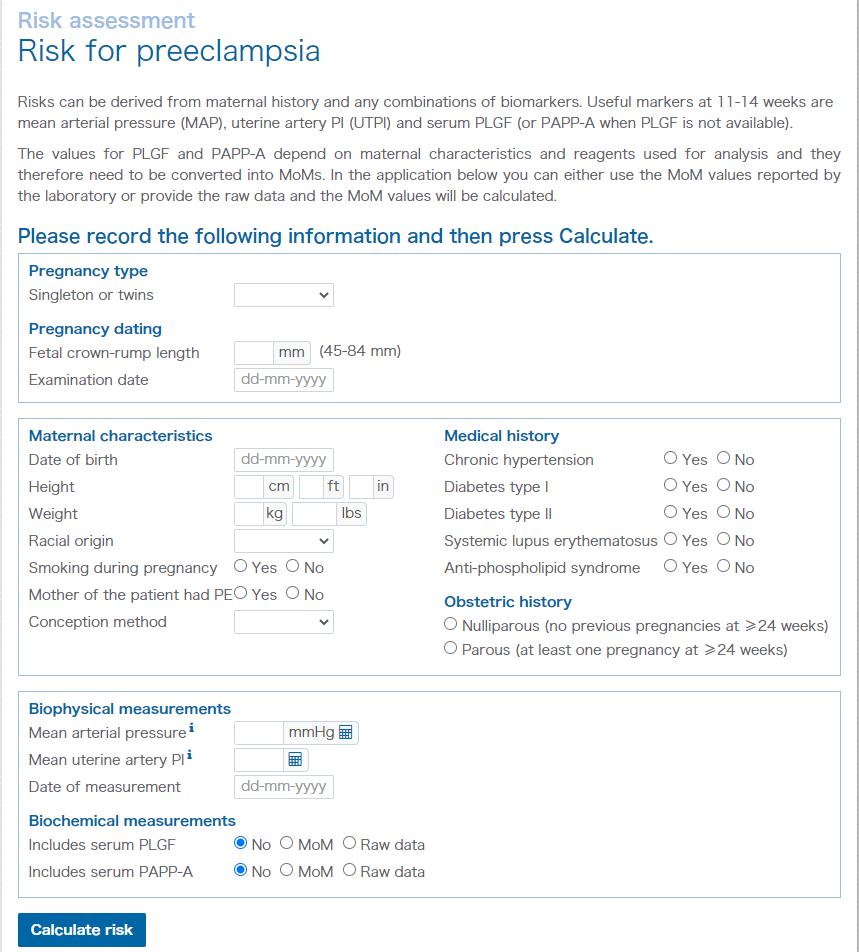
\includegraphics[width=.8\linewidth]{intro/risk}
    \caption[英国胎儿医学基金会使用的PE风险因子评估量表示意图]{\label{fig:risk}英国胎儿医学基金会使用的PE风险因子评估量表示意图\cite{risks}}
\end{figure}

\begin{longtblr}
    [
        theme          = {zju},
        caption        = {常见的PE风险因子汇总表},
        label          = {tab:riskfactors},
    ]
    {
        colspec        = {X[1,c,m]X[2.5,c,m]X[12,c,m]},
        hline{1,Z}     = {\thickline},
        hline{2}       = {\thinline},
        rowhead        = 1,
        row{odd}       = {bg=\oddcolor}, 
        row{even}      = {bg=\evencolor},
        row{1}         = {font=\headfont,bg=\headcolor},
        row{2-Z}       = {font=\nonheadfont},
    }
    序号 & 风险因子    & 可能的影响 \\
    1   & 妊娠年龄    &  PE的病发可能随妊娠年龄升高而增加\cite{Duckitt2005,FIGO,Yogev2010,Poon2010}。    \\
    2   & 胎产次/既往史&    首次分娩孕妇的PE病发可能比无PE既往史的二胎孕妇大\cite{Lee2000,Duckitt2005,Coonrod1995,Robillard1993,Sonia2009}。   \\
    3   & 妊娠间隔 & 多次妊娠的间隔时间过长或过短都会在一定程度上增加PE发生的风险\cite{Rousso2002,Duckitt2005,Conde2007,Mignini2016,Rolv2002}。\\
    4   & 辅助生殖 & 通过辅助生殖技术受孕的孕妇的PE病发可能增加\cite{Jackson2004,Trogstad2009,Martin2016}。\\
    5   & 家族史 & PE在一定程度上显现出家族性易感性\cite{ARNGRIMSSON1990,OAG9,Williams2011,Cincotta1998,FIGO}。\\
    6   & 肥胖 & 若孕妇出现肥胖症状(BMI>30$kg/m^2$),其PE病发风险会增加\cite{Duckitt2005,Williams2011,FIGO,Zintzaras2006,Sebire2001}。\\
    7   & 种族&不同民族、区域、肤色的孕妇的PE病发可能存在一定的差异\cite{Ghosh2014,Khalil2013}。\\
    8   & 并发症 & 当孕妇已患有某些疾病或感染某些症状时,其PE病发可能也会增加\cite{FIGO,Ray2016,OAG9,Lee2000,Garner1990,Martinell1990,Stamilio2000,Dreyfus2001,Marchetti2016}。\\
\end{longtblr}

二、生物标志物筛查

除上述量表外,另一种筛查PE的方法将孕妇的PE风险因子、特定病史的先验风险及其多项生物物理、生物化学检测结果相结合,基于贝叶斯定理估计该孕妇的PE病发风险\cite{FIGO}。
这一过程应用了参数估计中的极大后验概率估计原理(maximum a posteriori,MAP)\cite{Qiu2012},通过观测值及观测值的所属类别的后验概率,判断当前值最可能属于哪一类别并进行分类决策。
如基于MAP的二分类过程可以表示为
\begin{equation}
    \label{equ:maxap}
    H_{x}=
    \left \{
    \begin{aligned}
        &H_{0},  P(H_{0}|x)&\ge P(H_{1}|x), \\
        &H_{1},  P(H_{0}|x)&<P(H_{1}|x),
    \end{aligned}
    \right.  
\end{equation}
其中,$P(H|x)$为观测值$x$属于$H$的后验概率。比较这两个概率哪一个大,就判定$x$属于哪个类别,即
当$x=x_0$时,若满足$P(H_{0}|x) \ge P(H_{1}|x)$,则判定为$H_{0}$;反之,判定为$H_{1}$\cite{Qiu2012}。

上述筛选过程中使用到的孕妇生理、生化检测结果统称为生物标志物。其中,生理检测参数主要包括BP、子宫动脉搏动指数(uterine artery pulsatility index, UTPI)等;生化检测参数则种类繁多,且新参数层出不穷\cite{Rene2008,Zhong2015,Zeisler2016,Rana2012}。
这里选取妊娠相关血清蛋白-A(pregnancy-associated plasma protein A,PAPP-A)与胎盘生长因子(placental growth factor,PLGF)为代表进行介绍。

1、BP

由于PE是妊娠期高血压疾病的一种,BP一直是临床用于PE监测、诊断的重要指标之一\cite{OAG9,HDASOM,2000s1}。在进行BP测量时,应至少对孕妇的同一手臂测量两次。若两次的测量结果的SBP超过140 mmHg和(或)DBP超过90 mmHg,则将该孕妇诊断为高血压;
对首次发现血压升高的孕妇,应至少间隔4 h后再次测量确认\cite{OAG9}。此外,国际妇产科联盟也推荐使用平均动脉压(mean arterial pressure,MAP)作为实际标定诊断中的筛查指标\cite{FIGO},其计算方法如\autoref{equ:map}所示
\begin{equation}
    \label{equ:map}
    \text{MAP}=\text{DBP}+(\text{SBP}-\text{DBP})/3
\end{equation}

Leona C.Y. Poon等\cite{Poon2008}对5590名单胎孕妇的一项研究表明,单独使用MAP检测PE的检出率为38\%;而将孕妇病史等风险因子与MAP结合使用时,PE的检出率可达63\%,其假阳性率为10\%。
Stamilio等\cite{Stamilio2000}的另一项研究也发现,孕妇在初次产前检查发现MAP大于90 mmHg与其PE病发的相关性显著。


2、UTPI

UTPI是国际妇产科联盟与妇产科超声学会推荐的对PE进行筛查的参数之一\cite{FIGO,Sotiriadis2019}。
UTPI本质上也是一种血液动力学参数,其基本定义与\autoref{equ:map}中的MAP类似\cite{Cnossen2008}
\begin{equation}
    \label{equ:utpi}
    \text{UTPI}=\frac{A-B}{M}
\end{equation}
其中,$A$为子宫动脉收缩期血液峰值流量,$B$为子宫动脉舒张末期血液流量,$M$为该期间内的血液平均流量。
\begin{figure}[htbp]
    \centering
    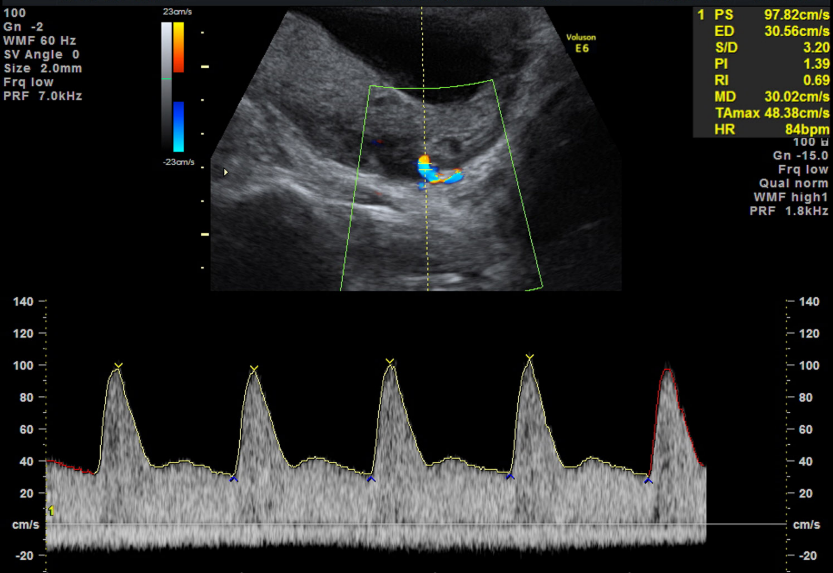
\includegraphics[width=.6\linewidth]{intro/utpi}
    \caption{\label{fig:utpi}子宫动脉的多普勒超声检查结果图}
\end{figure}

\autoref{fig:utpi}展示了一例孕早期经腹多普勒超声检查子宫动脉的结果\cite{Sotiriadis2019}。
常与UTPI一起使用的检测参数还包括子宫动脉阻力指数(uterine artery resistance index,UTRI)、子宫动脉收缩压/舒张压比(systolic to diastolic ratio,SDR)及切迹相关参数等\cite{Cnossen2008}。
Jeltsje S. Cnossen等\cite{Cnossen2008}的一项回顾研究表明,在孕妇妊娠$11^{+0}-13^{+6}$周时,若其UTPI数值上升或出现子宫动脉舒张早期切迹等现象,则该孕妇PE病发的可能性将增加\cite{OAG9,Plasencia2008}。

3、PAPP-A

PAPP-A是一种由细胞滋养层分泌的金属蛋白胰岛素生长因子结合蛋白,在胎盘的生长发育中起着重要的作用。PE已被证明与低水平的PAPP-A循环有关\cite{FIGO},但相关临床研究表明,仅使用PAPP-A单指标无法准确预测PE\cite{Smith2002}。
因此,PAPP-A常与其他检测参数一起配合使用\cite{Poon2009,Tan2018,Ray2018}。 

4、PLGF

PLGF是由绒毛状细胞滋养层膜细胞滋养层合成的一种糖基化二聚糖蛋白,具有血管生成合血管修复的功能。临床研究显示,PLGF的血管生成功能在妊娠过程中发挥很大作用,PLGF水平或其抑制受体水平的变化可能与PE的病发有关\cite{Levine2004,Ahmad2004}。
同时,临床证据表明,在孕早期患有PE的孕妇其PLGF的浓度较正常妊娠孕妇更低\cite{Chau2017}。

2015年,Zhong等\cite{Zhong2015}对多项血清生化指标在PE预测方面的性能进行了比较,结果显示,PLGF的综合性能优于PAPP-A等其他血清生化指标。
2019年,Duhig等\cite{Duhig2019}对多名疑似PE的孕妇进行了追踪实验,持续性地检测孕妇的PLGF水平(总实验人数$N$=1019,实验组人数$N_{PE}$=573,对照组人数$N_{Control}$=446,下同)。
结果显示,实验组的PE诊断时间的中位数为4.1天,而对照组仅为1.9天,这证明PLGF可以有效缩短PE确诊的时间。
鉴于此,FIGO组织特别将胎盘生长因子推荐为PE检测首选生化指标\cite{FIGO}。

\subsection{医用检测设备}
本小节将从现阶段在临床使用的标准医疗设备与新兴微型化智能设备等两个方面对PE检测设备进行介绍。

一、标准医疗设备

目前临床所使用的PE筛查检测设备主要以检测生化标志物为主,国内外医疗器械公司均研发推出了一系列的软硬件综合分析系统。但整体而言,国内医疗器械设备公司研发起步晚,可检测指标数目也更少。

1、德国Thermo Fisher Scientific公司的产前检测设备

德国Thermo Fisher Scientific公司一直致力于对各种生物标志物检测的研究,其公司BRAHMS系列的KRYPTOR GOLD与KRYPTOR compact PLUS等型号设备可对多种生物标志物的进行检测\cite{B·R·A·H·M·S2023}。
除PAPP-A与PLGF外,这些设备还可对游离雌三醇(unconjugated estriol, uE3)、甲胎蛋白(alpha fetoprotein,AFP)、人绒毛膜促性腺激素(human chorionic gonadotropin,HCG)及
可溶性fms样酪氨酸激酶-1(soluble fms like tyrosine kinase 1,sFlt-1)等多种PE生物标志物进行检测,
可应用于PE的早期筛查及诊断等多种场景,如\autoref{fig:B·R·A·H·M·S}所示。
同时,该公司还提供了与硬件配套的Fast Screen pre I plus$^\text{TM}$综合软件分析系统,可结合硬件设备的检测结果对孕妇PE病发可能进行全面地风险评估。

\begin{figure}[htbp]
    \centering
    \subfigure[KRYPTOR GOLD]{
    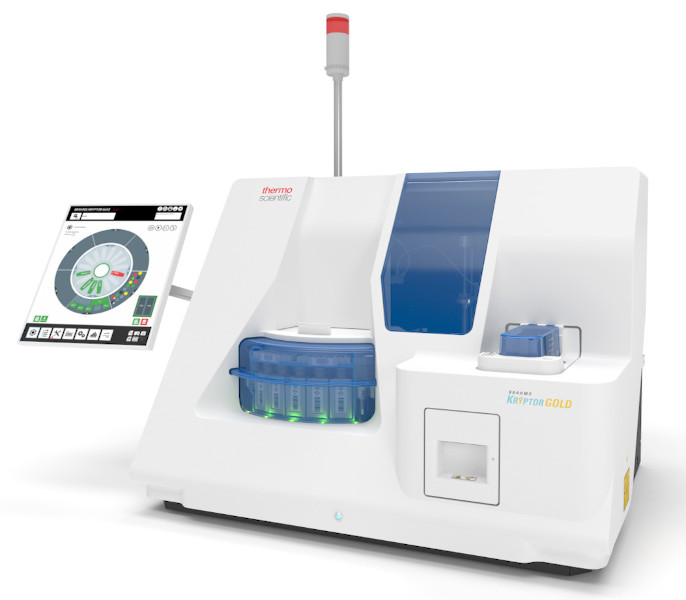
\includegraphics[width=5cm]{intro/brahms-kryptor-gold-686}
    }
    \quad
    \subfigure[KRYPTOR compact PLUS]{
    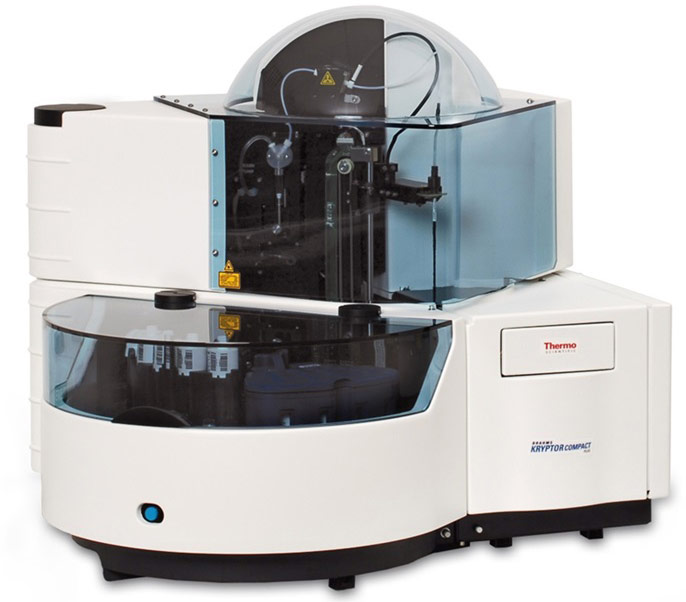
\includegraphics[width=5cm]{intro/brahms-kryptor-compact-plus-686}
    }
    \caption{\label{fig:B·R·A·H·M·S}德国Thermo Fisher Scientific公司的KRYPTOR检测设备示意图}
\end{figure}
\vspace{1cm}
\begin{figure}[htbp]
    \centering
    \subfigure[VICTOR2$^\text{TM}$ D荧光检测仪]{
    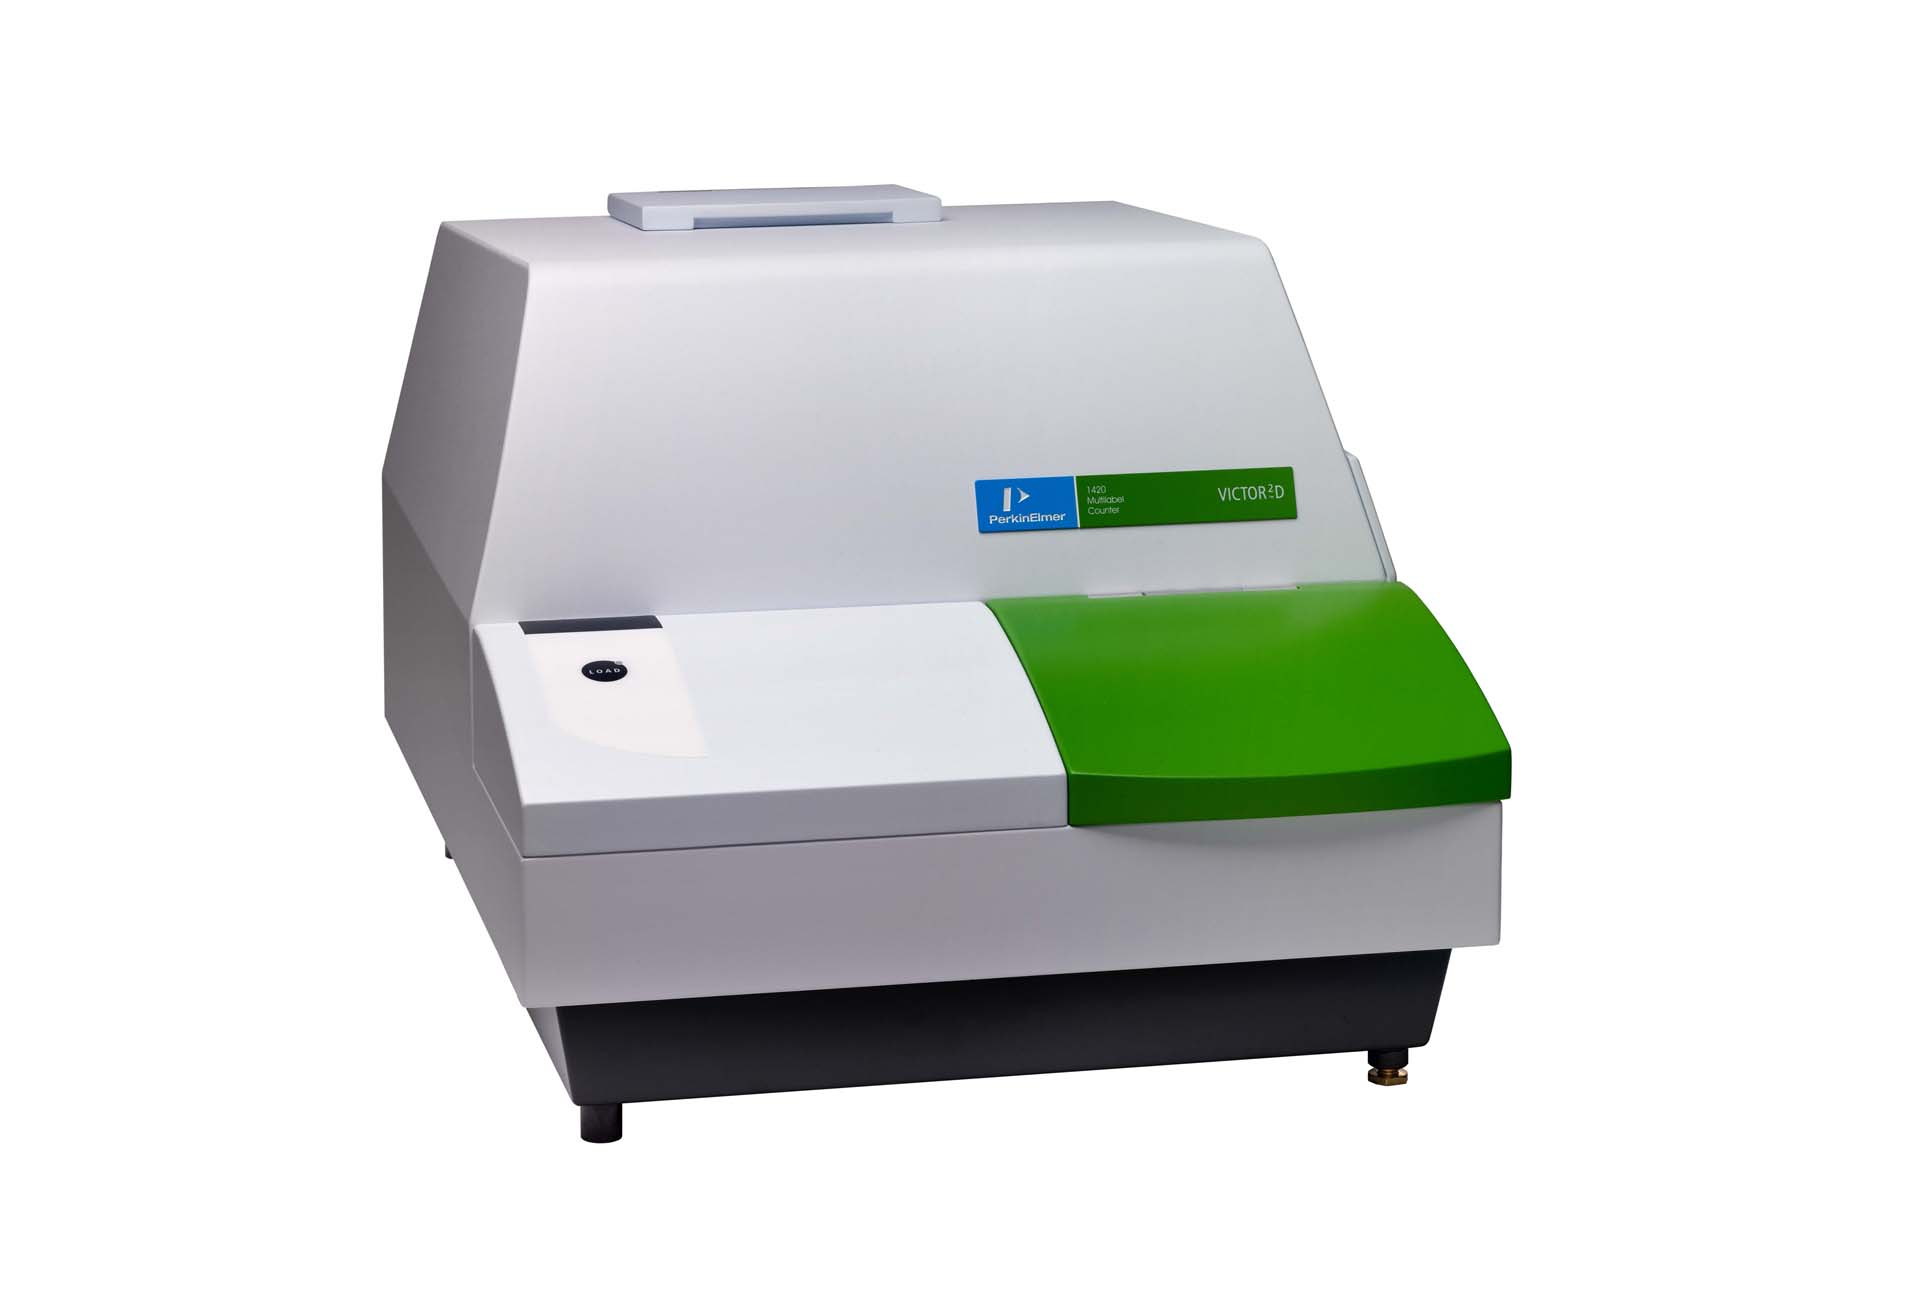
\includegraphics[width=5cm]{intro/Victor-2D-72ppi}
    }
    \quad
    \subfigure[DELFIA$^\circledR$ Xpress免疫分析仪平台]{
    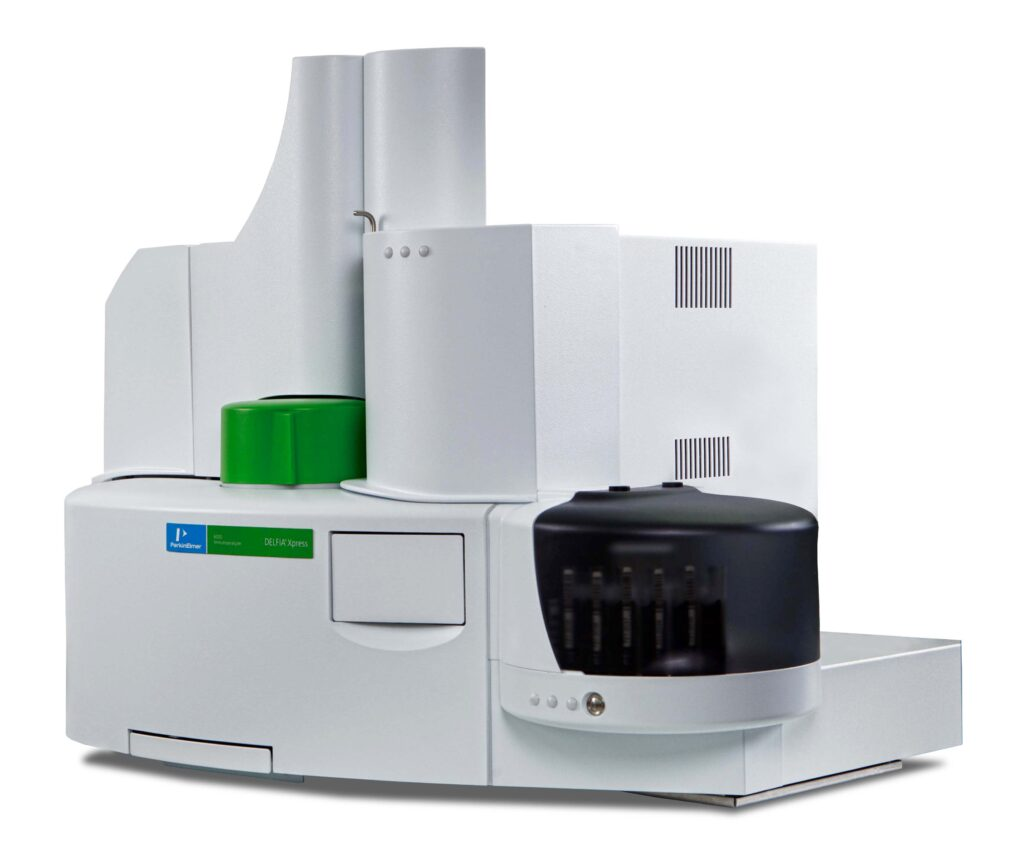
\includegraphics[width=5cm]{intro/dx}
    }
    \caption{\label{fig:PerkinElmer}美国PerkinElmer公司的免疫荧光检测设备示意图}
\end{figure}
\vspace{1cm}

2、美国PerkinElmer公司的产前检测设备

为推进早期检测在临床医疗领域的应用,美国PerkinElmer公司也提供了较为全面的筛查和诊断解决方案组合\cite{perkinelmer2023}。该公司的AutoDELFIA$^\circledR$、
DELFIA Xpress$^\circledR$及VICTOR2$^\text{TM}$等系列免疫荧光分析仪平台,可应用于多种孕期综合并发症的临床检测之中,如\autoref{fig:PerkinElmer}所示。这些设备可对包括AFP、hCG、PAPP-A、PLGF、
sFlt-1、uE3等在内的多种PE生物标志物进行检测标定。此外,该公司也配套研发了LifeCycle$^\text{TM}$软件分析系统,可实现从样品接收、检验检测、风险评估及产出综合报告的全自动分析工作流程。

3、中国宁波奥丞生物科技有限公司的荧光检测设备

作为中国新兴的医疗器械设备公司,宁波奥丞生物科技有限公司致力于提供专业的妇幼健康临床诊断解决方案,力求通过提供可靠、快速与便捷的体外诊断产品为临床诊疗提供精准的检测结果。
目前,宁波奥丞生物科技有限公司提供了微小型床边诊断设备与大型实验室标定两种类型的设备,多款化学荧光免疫平台产品均支持对PE生物标记物PLGF与sFlt-1的检测
,如\autoref{fig:aucheer}所示\cite{aucheer2023}。
\begin{figure}[h]
    \centering
    \subfigure[微流控荧光免疫定量检测系统 iSort300]{
    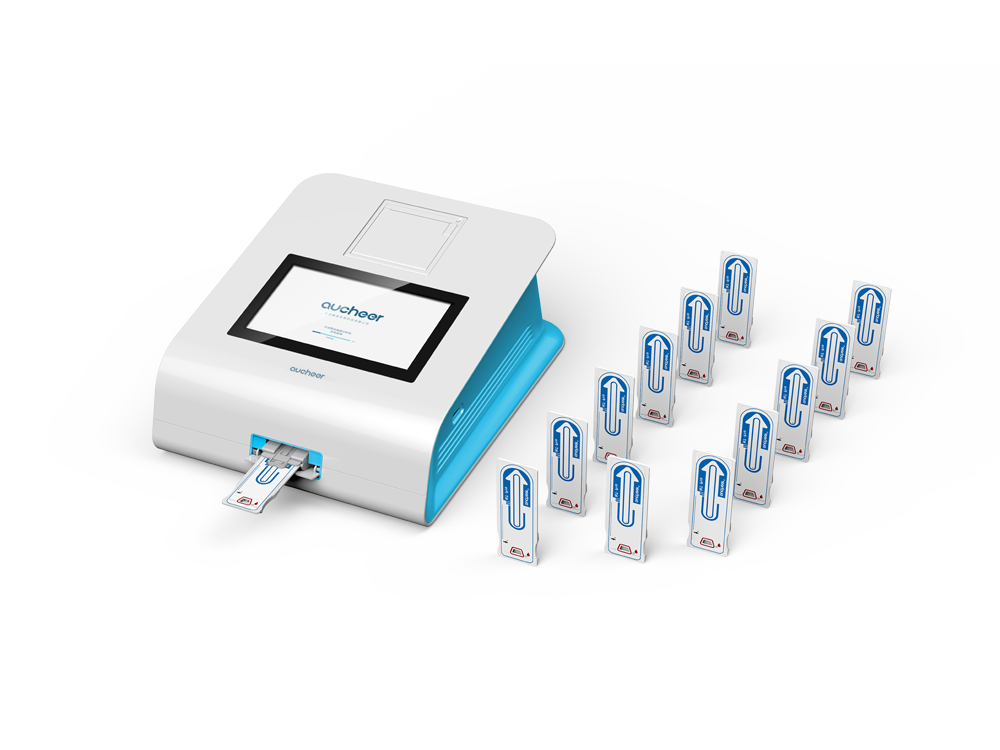
\includegraphics[width=6cm]{intro/isort300}
    }
    \quad
    \subfigure[全自动化学发光免疫检测系统 Shine i1910]{
    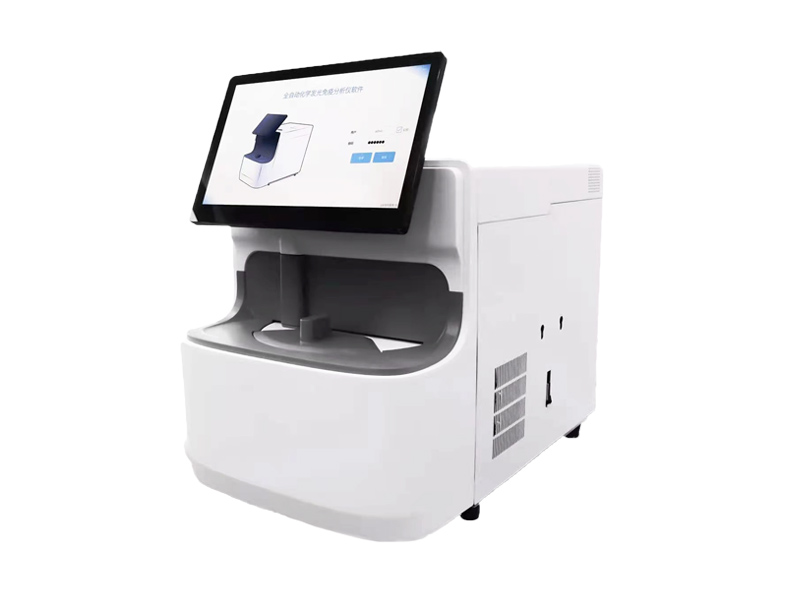
\includegraphics[width=6cm]{intro/shinei1910}
    }
    \caption{\label{fig:aucheer}中国宁波奥丞生物科技公司的荧光免疫检测设备示意图}
\end{figure}

二、微型智能设备

近年来随着移动智能医疗和可穿戴式设备的发展,通过微型智能设备实现PE相关指标的实时、动态、多场景检测也逐渐成为了新的研究热点。
但整体而言,PE的微型智能检测设备仍处于研发阶段,能真正实现多场景检测的成熟产品尚未出现。

2019年,Iuliana Marin等\cite{Marin2019,Marin2020}通过一款智能腕部血压检测穿戴设备对孕妇的血压数据进行了监测。他们在综合考虑孕妇的年龄、体重等风险因素的基础上,通过维特比动态规划算法(Viterbi algorithm,VB),分析孕妇的PE
病发可能,该分析系统原理框架图如\autoref{fig:mobile}所示。Iuliana Marin团队利用该系统
对多名孕妇进行了测试($N$=105)。结果显示,最终的生成模型可以达到总体准确率80.0\%,其中敏感性为92.5\%,特异性为72.0\%\cite{Marin2019}。
\begin{figure}[htbp]
    \centering
    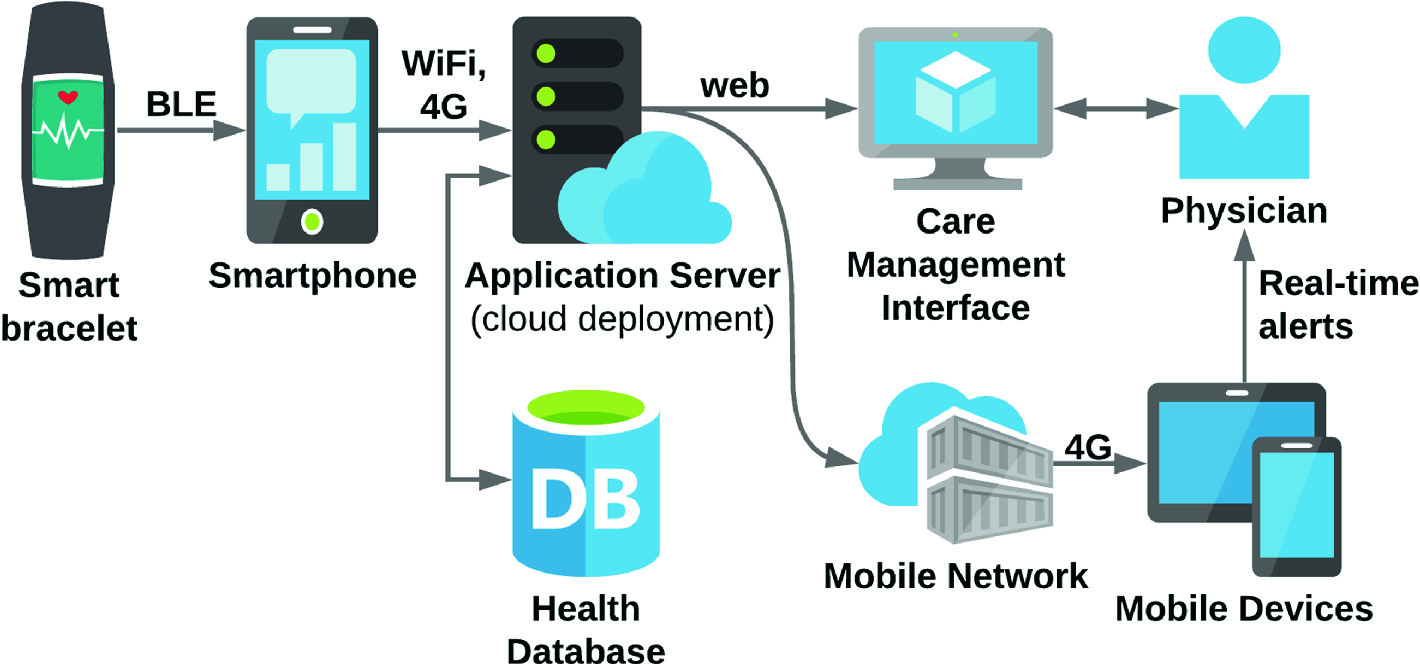
\includegraphics[width=.7\linewidth]{intro/mobile}
    \caption[基于智能穿戴设备的血压检测系统框架图]{\label{fig:mobile}基于智能穿戴设备的血压检测系统框架图\cite{Marin2019,Marin2020}}
\end{figure}

\subsection{人工智能检测技术}
随着现代化医学检测设备的普及与医学信息化技术的发展,医学诊断过程中也开始涌现出海量检测数据。这些激增的数据也促进了计算机领域机器学习(machine learning, ML)技术在医学相关问题上的创新应用与发展。
近年来,专家学者们也逐渐开始将ML技术应用于PE的识别、判断及预测的研究中。这些研究可按应用研究方向大体分为数据挖掘与分类聚类分析等两大类\cite{Mehta2016}。

一、数据挖掘

数据挖掘,又称为关联规则,力求发现多项数据之间的隐藏的逻辑与关系\cite{Han2006}。利用数据挖掘技术从血浆代谢物、蛋白质及RNA等生化指标中筛选出与PE病发相关性较强的成份一直是PE的热点研究方向。
这些研究在实现了数据降维的同时,也揭示了数据之间隐藏的联系。

2005年,Louise C. Kenny等\cite{Kenny2005}利用基因遗传算法(genetic programming, GP),通过血浆中特定代谢物成份来识别PE病发的孕妇($N_{PE}$=87,$N_{Control}$=87)。
他们通过GP算法训练得到了仅使用三种代谢物峰值变量的PE预测模型。经验证,该模型可以较好地区分PE病发孕妇与正常孕妇,其灵敏度高达100.0\%,特异性高达98.0\%。

2018年,Liron Yoffe等\cite{Yoffe2018}为寻找能有效区分识别PE的转录RNA,对孕妇妊娠前三个月的血浆中的非编码循环RNA丰度进行了分析($N_{PE}$=75,$N_{Control}$=75)。在对非编码RNA测序后,他们确定了实验组与对照组
之间差异表达的25个RNA,并在此基础上训练生成了一个逻辑回归预测模型。经验证,通过受试者工作特征曲线(receiver operating characteristic,ROC)得到该模型的曲线下面积(area under curve,AUC)数值可达0.86。

2018年,Muhlis Tahir等\cite{Tahir2018,Tahir2018-2}对比了神经网络(neural networks, NN)和深度学习(deep learning, DL)两类算法预测妊娠期孕妇PE病发风险水平的结果($N$=1077)。
他们使用粒子群优化(particle swarm optimization, PSO)算法进行特征选择,将原始数据集的17个参数缩减至9个。
经留一法(leave one out,LOO)验证表明,当使用NN算法训练模型时,在原始数据集上训练的模型识别准确率为93.2\%,而在缩减后的数据集上模型的准确性为93.8\%。
当使用以人工神经网络(artificial neural network,ANN)为代表的DL算法在两个数据集上训练所得模型的准确性分别为95.1\%与95.7\%。
两者的数值差异可能与ANN较NN具有更多隐藏层、网络的整体结构更加复杂等因素有关。

2020年,Jose F Carre˜no等\cite{Carreno2020}基于蛋白质组学数据,比较了降维(dimension reduction,DR)与时间序列总结(time-series summary,TSS)两类算法对PE的预测的效果($N$=202)的影响。
他们使用了帝国竞争与基因集簇两种DR算法,全局平均与三点平均(对应孕前中晚期数据)两种TSS算法。
经验证,两类算法在两个独立数据集上均达到了约90.0\%的准确性;较孕晚期的蛋白质组学数据而言,使用孕早期与孕中期的数据进行PE预测的结果会更准确。

2021年,Yixin Li等\cite{LI2021102}通过逻辑回归(logistic regression,LR)、随机森林(random forest,RF)、支持向量机( support vector machines,SVM)和极限梯度提升(extreme gradient boosting,XGBoost)
等算法对孕早期和孕中期孕妇的电子病历进行了分析,从38个临床参数中构建了PE的识别模型($N$=3759) 。
其研究结果表明,由极限梯度提升算法生成的模型具有最佳的预测性能,其准确率为92.0\%,精确度为44.7\%,AUC为0.96。

2023年,Hao Wang等\cite{HW2023}设计了一种计算生物学方法,从单细胞转录组(scRNA-seq)来识别病理细胞亚群并预测孕妇的PE病发风险($N_{PE}$=7970,$N_{Control}$=7178)。
他们的结果表明,将极限梯度提升算法与ReliefF特征选择算法结合使用时,可以取得最优的识别模型性能。通过最佳模型对健康胎盘的九个细胞亚群进行分类,可达到92.6\%的准确率与92.5\%的召回率。

二、 分类与聚类分析

分类分析(classification)是按照某种标准给对象一定的数据标签,再根据数据标签来区分归类的过程,即通过现有数据建立模型预测新数据所属类别的过程。
而聚类分析(clustering)则是在没有数据标签的情况下,按照一定规则将所有数据分组,
使每组内的数据尽可能相似并有别于其他组数据的过程\cite{Han2006}。
分类分析与聚类分析是PE在ML领域最活跃的方向,而PE风险因子则是分类与聚类分析下使用得最为广泛的研究数据。

2017年,Pia M. Villa等\cite{Villa2017}应用贝叶斯聚类(Bayesian clustering,BC)算法,通过PE风险因子对受试孕妇进行了分析($N$=903),并计算了聚类得到的各簇PE病发可能。
结果表明,PE的病发可能随孕妇PE风险因子数量增加而指数增长。同时,PE病发的程度也往往随孕妇风险因子的种类差异而呈现不同。

2020年,Ivana Mari{\'{c}}等\cite{Maric2020}利用弹性网(elastic net,EN)算法与梯度提升(gradient boosting,GB)算法,基于67项PE风险因子训练得到了PE预测模型与早发PE预测模型($N$=16370)。
经验证,PE预测模型的AUC数值可达0.79,识别假阳性率为8.1\%;早发PE预测模型的
AUC高达0.89,真阳性率为72.3\%,假阳性率为8.8\%。

2020年,Herdiantri Sufriyana等\cite{Sufriyana2020-1}使用多种ML算法,基于多项PE风险因子与包括sFlt-1、UPTI与PLGF的多项生化指标对孕妇的PE病发可能进行了研究($N_{PE}$=66,$N_{Control}$=29)。
他们发现利用决策树(decision tree,DT)算法得到的PE识别模型具有最佳分类效果,可实现100\%的识别精确度与95\%的敏感度。在最佳识别模型下,贡献度较大的的特征包括体重、BMI、UPTI、sFlt-1、PLGF及sFlt-1与PLGF比值等。
同年,Sufriyana团队也就上述风险因子与生化指标与PE相关性进行了研究\cite{Sufriyana2020}。他们在来自印度尼西亚孕妇的包含95个特征的数据集上建立了PE识别模型($N_{PE}$=3318,$N_{Control}=$19883)。结果表明,
由17项特征生成的随机森林模型对PE具有最好的预测分析效果。

% 2022年,郑江元\cite{ZJY2022}等采用单因素分析与逻辑回归相结合的方法,从孕妇的45项风险因子中筛选出了12项指标,在此基础上使用轻量的梯度提升机(Light Gradient Boosting Machine,LGBM)构建了PE的识别模型($N_{PE}$=291,$N_{Control}$=1318)。
% 他们运用5折交叉验证的方法确定LGBM算法的最优参数,最佳模型的AUC数值为0.964,灵敏度为0.849,特异度为0.927,精度为0.716。

2022年,Leon J. Schmidt等\cite{SCHMIDT202277}分析了孕妇的sFlt-1、PLGF与多项超声检测数据(包括脐动脉脉动指数、大脑中动脉脉动指数、平均子宫动脉脉动指数等),构建了114个特征($N$=2472)。随后,他们
使用了梯度增强树(gradient-boosted tree,GBT)与随机森林算法进行了PE识别模型的训练。结果表明,梯度增强树模型的阳性预测值为88.0\%±6.0\%,阴性预测值为89.0\%±3.0\%,灵敏度为66.0\%±5.0\%,特异性为
97.0\%±2.0\%,
\begin{landscape}
    \begin{longtblr}
        [
            theme          = {zju},
            caption        = {人工智能检测技术在PE领域的研究汇总表},
            label          = {tab:AIinPE},
            note{*}        = {由于篇幅限制,该研究未在正文中进行介绍,具体研究内容请参阅原文。},
        ]
        {
            colspec        = {X[0.8,c,m]X[0.8,c,m]X[4.5,c,m]X[2,c,m]X[5,c,m]X[5,c,m]X[2,c,m]},
            hline{1,Z}     = {\thickline},
            hline{2}       = {\thinline},
            rowhead        = 1,
            row{odd}       = {bg=\oddcolor}, 
            row{even}      = {bg=\evencolor},
            row{1}         = {font=\headfont,bg=\headcolor},
            row{2-Z}       = {font=\nonheadfont},
        }
        序号 & 时间 & 研究者 & 主要任务 & 涉及的机器学习方法 & 涉及参数 & 数据规模 \\
        1 & 2005&Louise C. Kenny\cite{Kenny2005}&降维、分类&基因遗传算法&多种血浆代谢物&174\\
        2 & 2009&Costas K. Neocleous\cite{Neocleous2009}\TblrNote{*}&降维、分类&神经网络&PE风险因子及生化指标&6838\\
        3 & 2016&Mário W. L. Moreira\cite{Moreira2016}\TblrNote{*}&降维、分类&贝叶斯网络&PE风险因子及多项生理症状&164\\
        4 & 2017&Pia M. Villa\cite{Villa2017}&聚类分析&贝叶斯聚类算法&PE风险因子&903\\
        5 & 2018&Muhlis Tahir\cite{Tahir2018,Tahir2018-2}&降维、分类&粒子群优化算法&PE风险因子&1077\\
        6 & 2018&Liron Yoffe\cite{Yoffe2018}&降维、分类&逻辑回归&非编码循环RNA&150\\
        7 & 2018&Antonieta Martínez-Velasco\cite{Martinez2018}\TblrNote{*} &分类&多种ML算法&PE风险因子及多项其他指标&1634\\
        8 & 2019&Jong Hyun Jhee\cite{Jhee2019}\TblrNote{*}&{模式识别、\\聚类分析}&{逻辑回归、决策树、\\朴素贝叶斯、随机森林等}&PE风险因子及多项其他指标&11006\\
        9 & 2020&Jose F Carre˜no\cite{Carreno2020}&降维、分类&{帝国竞争算法、基因集簇算法、\\时间序列总结算法}&多种蛋白质组学物质&202\\
        10 & 2020&Ivana Mari{\'{c}}\cite{Maric2020}&分类&弹性网算法&PE风险因子&16370\\
        11 & 2020&Oknalita Simbolon\cite{Simbolon2020}\TblrNote{*}&分类&投票&PE风险因子&402\\
        12 & 2020&Herdiantri Sufriyana\cite{Sufriyana2020-1}&分类&决策树&PE风险因子及生化指标&95\\
        13 & 2020&Herdiantri Sufriyana\cite{Sufriyana2020}&降维、分类&随机森林算法&PE风险因子及多项其他指标&23201\\
        14 & 2021&Rong Guo\cite{Guo2021} \TblrNote{*} &降维、分类&{集成学习、 决策树、\\自适应增强、多层感知机}&胎盘mRNA&330\\
        15 & 2021&Yixin Li\cite{LI2021102}&降维、分类&{逻辑回归、 随机森林、\\支持向量机、极限梯度提升}&PE风险因子及多项其他指标&3759\\
        16 & 2022&Leon J. Schmidt\cite{SCHMIDT202277}&降维、分类&梯度增强树、随机森林算法&sFlt-1、PLGF与多项超声检测数据&2472\\
        17 & 2022&Ansbacher-Feldman\cite{Ansbacher2022}&降维、分类&随机森林算法&PE风险因子、疾病史与生物标志物&60789\\
        18 & 2023&Hao Wang\cite{HW2023}&降维、分类&极限梯度提升&单细胞转录组&15148\\
    \end{longtblr}
\end{landscape}

\noindent
总体准确度为89.0\%±3.0\%;而随机森林模型的阳性预测值为88.0\%±6.0\%,特异性为97.0\%±1.0\%,其他指标表现稍差。

2022年,Ansbacher-Feldman等\cite{Ansbacher2022}分析了孕妇的PE风险因子、疾病史与UTPI、MAP、
PLGF及PAPP-A等四种生物标志物的检查结果,使用神经网络算法对其PE病发风险进行了预测($N$=60789)。结果表明,
仅通过孕妇的风险因子筛查时,PE检出率为53.3\%,相应的AUC为0.82;而将生物标志物加入模型后,这些数值可分别增加到75.3\%和0.91。

\autoref{tab:AIinPE}总结了近年来ML技术在PE识别、分析及预测等相关问题的多项研究。从\autoref{tab:AIinPE}可以发现,
利用ML技术分析PE风险因子、生物标志物等参数是目前炽手可热的多学科交叉研究点。

\subsection{存在的不足与分析}
综合上述分析,随着近年来临床对PE的了解不断深入,现阶段PE已经具有较为成熟的识别技术与检测手段。借助专业的检测仪器设备获取数据,通过风险因子与生物标记物筛查等方法,
可以对PE进行较高准确率地识别与诊断。但上述检测方法仍然存在着一定的缺陷与不足。

一、风险因子筛查

整体而言,风险因子可以对孕妇PE的病发可能性进行一定程度上的初筛,但其准确性有限。此外,风险因子往往是对孕妇某些特性的静态描述,无法体现
整个孕期内的任何动态变化,具有一定的滞后性。

二、生物标志物筛查

生物标志物筛查较风险因子对PE的识别与诊断有着更高的准确性与可靠性,但这些生物标志物(如sFlt-1、UPTI与PLGF等)必须借助专业设备在医院进行有创采样检测,
对检测设备与场所、操作设备流程等多方面均有一定要求且成本较高。

三、人工智能检测技术

如\autoref{tab:AIinPE}所示,此前诸多学者虽然应用机器学习方法对PE相关问题进行了一定的分析,但数据来源主要为蛋白质、mRNA等生物标志物
。这些生物标志物类数据的获取有着较大的难度与较高的专业壁垒。
% 而获取方便的人体电生理信号等指标很少出现在此类研究中。

鉴于现有技术存在上述不足,实现对PE的便捷、快速、无创、准确的临床诊断乃至全孕期内的动态监测无疑有着广阔的研究空间与应用前景。
针对PE的识别与检测,可按以下思路进行研究:

一、寻求更好的能够表征PE的参数指标

寻求更好的能够表征PE的参数指标无疑是后续分析研究得以开展的基础,
根据现有的PE的病发机制与理论,PE会导致孕妇多器官、多系统的病生理变化。因此,从这些受影响的器官、系统中挖掘出能够表征PE病发的新特征参数具有理论可能性与实践可行性。

二、利用机器学习领域的相关算法建立更好的分析模型

将现有的机器学习分析技术应用到PE的识别的具体问题中,综合使用多种机器学习模型、算法对上述指标数据进行分析,最终得到PE识别模型。

另一方面,光电容积脉搏波(photoplethysmography, PPG)是心脏周期性搏动的体现,包含了有关人体血液微循环方面的更富细节的生理信息\cite{PPGYY}。
由于血管直径富于变化,PPG到达之处血液流动速率也将发生一定的脉动变化。而PE会引起全身小动脉痉挛,必然会引起血液动力学上的变化,因此,这些变化理论上可以从PPG上得到体现。
而PPG在采集测量过程中定位简单、易于操作,具有无创、无痛、迅速、便捷等优点,采集得到的信号质量高、稳定性强,
在观察和评估微循环状况上具有天然优势,是临床各类监护设备必备的监测参数之一,已在动脉硬化、高血压、心肌梗塞等心脑血管疾病上得到了一定的应用
\cite{PPGYY,Allen2007,THOCBPM,Zhang2010,ldl,lhc}。

\textbf{鉴于此,本研究使用PPG信号提取特征,利用多种机器学习算法对PE的识别进行相关研究。}

\subsection{脉搏波在子痫前期领域的研究现状}
近年来,学者们基于PPG数据也对PE进行了一定的研究。本小节将按传统指标与新型指标两大类对这些研究进行介绍,其中,传统指标指已经在其他领域的基于PPG的研究中得到广泛应用的特征参数;而新型指标特指
近年来在PE研究领域被相关学者新提出的PPG特征参数。本节出现的参数的具体定义可参见第三章内容。

一、传统指标

2008年,Karlijn Vollebregt等\cite{KARLIJN2008}研究了使用PPG数据进行PE初筛的可能。他们通过对健康孕妇的跟踪研究表明,舒张压、心输出量与PPG增强指数(augmentation index,AIX)
均对PE预测模型有明显影响($N$=223)。

2012年,Kathleen Tomsin等\cite{Tomsin2012}对静脉PPG传播速度(pulse wave velocity,PWV)进行了研究。研究结果显示,在正常妊娠期孕妇所有脏器的PWV均呈现逐渐升高的趋势。
但PE早期($N$=12)及晚期患者($N$=14)的PWV数值较正常孕妇($N$=16)数值更低。Ira Bernstein等\cite{Ira2014}、Mihaela Viviana Ivan等\cite{VivianaIvan2018}及Irene Katsipi等\cite{Katsipi2014}
的多项研究也进一步验证PWV在PE检测识别中的作用。

2013年,Maximilian B. Franz等\cite{Franz2013}研究发现正常孕妇的AIX数值在孕期会出现内先下降再升高的现象,而早发和晚发的PE孕妇在妊娠期间AIX数值明显增高,且早发PE孕妇即使在产后AIX与PWV数值均明显升高
($N_{PE}$=21,$N_{Control}$=35)。

2014年,Su Fangming等\cite{Su2014}研究发现,通过PPG可以无创评估整个妊娠过程中心血管活动情况。他们提取分析了PPG增强指数、反射指数(reflection index,RI)、脉搏传导时间(pulse transit time,PTT)等,
发现这些参数随着妊娠进行在孕期内均有统计意义上的明显改变。

2014年,Nan Han等\cite{Han2014}对孕妇心血管系统与子宫动脉血流系统的一致性进行了研究,也得到了与Kathleen Tomsin等\cite{Tomsin2012}类似的结论。他们以三个月为单位对子宫动脉多普勒超声与指端PPG的检测结
果进行了对比分析($N_{PE}=$10,$N_{Control}=$80)。结果显示,正常孕妇的UTRI与RI均随妊娠进行而显著降低,且趋势基本一致;而PE患者的两项参数数值均明显高于正常孕妇。

2018年,Tammy Y. Euliano等\cite{Euliano2018}通过心电与PPG对识别PE患者($N_{PE}$=37,$N_{Control}$=43)进行了研究。他们发现PE患者的相邻PPG波峰间期较正常孕妇长、弹性系数较正常孕妇小。

二、新型指标

2018年,Ying Feng等\cite{Feng2018}提出了PPG的差异面积比参数(area difference ratio,ADR),并对72例孕妇($N_{PE}$=36,$N_{Control}$=36)的PPG数据进行了评估。
结果表明,PE病发孕妇的ADR数值较正常妊娠孕妇低。

2019年,陈婉琳等\cite{Chen2019}提出了PPG的光电容积斜率指数(photoplethysmography slope index,PSI),并对50例孕妇($N_{PE}$=23,$N_{Control}$=27)的PPG数据使用PSI进行了检验。
结果表明PSI区分PE的准确性达到 92.0\%,灵敏性为87.0\%,特异性为96.3\%。

以上基于机器学习的PE研究可总结为\autoref{tab:PPGinPE}所示。
从\autoref{tab:PPGinPE}可知,PE患者的血流动力学变化与PPG之间确实存在着一定的联系,但此前的各项研究在使用的PPG特征指标与分析方法上均有一定的局限性。
除AIX、PTT、PWV等传统参数之外,更多PPG特征参数有待进一步挖掘;而此前介绍过的各项机器学习算法在PPG与PE的研究上也有待开展探索。

\begin{longtblr}
    [
        theme          = {zju},
        caption        = {基于PPG的PE研究汇总表},
        label          = {tab:PPGinPE},
    ]
    {
        colspec        = {X[0.8,c,m]X[0.8,c,m]X[3.4,c,m]X[1.8,c,m]X[7.7,c,m]},
        hline{1,Z}     = {\thickline},
        hline{2}       = {\thinline},
        rowhead        = 1,
        row{odd}       = {bg=\oddcolor}, 
        row{even}      = {bg=\evencolor},
        row{1}         = {font=\headfont,bg=\headcolor},
        row{2-Z}       = {font=\nonheadfont},
    }
    序号 & 时间 & 研究者 & PPG参数 & 主要研究结论 \\
    1  & 2008    &   Karlijn Vollebregt\cite{KARLIJN2008}    &   AIX     &   AIX对PE预测模型有明显影响。\\
    2  & 2012    &   Kathleen Tomsin\cite{Tomsin2012}    &   PWV     &   PE患者的PWV数值较正常孕妇数值更低。 \\
    3  & 2013    &   Maximilian B. Franz\cite{Franz2013}    &   AIX     &   PE患者与正常孕妇的AIX数值在孕期内规律不一致。 \\
    4  & 2014    &   Ira Bernstein\cite{Ira2014}     &   PWV &  PE患者的PWV数值较正常孕妇数值更低。 \\
    5  & 2014    &   Irene Katsipi\cite{Katsipi2014}     &   PWV &  PWV是预测PE的一个潜在的有利因素。 \\
    6  & 2014    &   Nan Han\cite{Han2014}     &   UTRI &  PE患者的UTRI数值明显高于正常孕妇。 \\
    7  & 2014    &   Su Fangming\cite{Su2014}    &   {AIX、RI、\\PTT}    &   这些参数在孕期内有统计意义上的明显改变。\\
    8  & 2018    &   Mihaela Viviana Ivan\cite{VivianaIvan2018}     &   PWV &  PWV数值与PE之前间存在正相关。 \\
    9  & 2018    &   Tammy Y. Euliano\cite{Euliano2018}     &   {PPG波峰\\间期、弹性\\系数} &   {PE患者的PPG波峰间期较正常孕妇长、\\弹性系数较正常孕妇小。}\\
    10  & 2018    &   Ying Feng\cite{Feng2018}    &   ADR &  PE患者的ADR数值较正常孕妇数值更低。 \\
    11  & 2019    &   陈婉琳\cite{Chen2019}     &   PSI & PSI可在一定程度上识别PE。  \\
\end{longtblr}

\section{研究目标与研究内容}

\subsection{研究目标}
基于PE病发与正常妊娠孕妇的PPG数据,从多种角度研发设计新型PPG形态学特征参数,构建通用的PPG时域特征集。
从PPG时域特征集筛选出与PE相关性强的特征参数,在此基础上,使用多种机器学习算法构建PE识别模型,并对模型的有效性与可靠性进行验证。
开发一款能够完成上述具体研究任务的PE识别分析软件系统。
\subsection{研究内容}
全文研究内容可分为临床实验数据获取、PPG信号的预处理、PPG新型时域特征参数设计、PPG时域特征描述集合构建、PE的识别模型的构建与评估
及基于PPG的PE识别分析软件系统的设计与实现等具体六个部分,每部分研究内容
包括:

一、临床实验数据获取

本研究所使用的PPG数据来源自自主进行的临床实验,对该临床实验流程、使用设备等进行介绍。对获取到的数据进行复核,同时对参与临床实验的被试的人口统计学特征进行分析。

二、PPG信号的预处理

完成PPG分析前的预处理工作,包括滤波处理、波形检测、重搏波与切迹检测、去除基线漂移、信号重采样与数据标准化等处理步骤。

三、PPG新型时域特征参数设计

对PPG时域特征的设计过程进行方法学的归纳,提出PPG特征描述向量,提出多种基于时间、幅值、角度、弧度、面积、斜率等多维度的新型PPG时域特征;
提出描述PPG波形间差异的新型时域特征。

四、PPG时域特征描述集合构建

在上述设计得到的新型时域特征参数中,选取与PE相关性强的特征参数,构建PPG时域特征描述集合。

五、PE的识别模型的构建与评估

在PPG时域特征集合的基础上,综合使用多种机器学习算法,训练构建PE的识别模型。基于已有的数据,对识别模型的性能进行评估,验证模型的可靠性。

六、PE识别分析软件系统的设计与实现

基于软件开发思想,综合利用多种软件开发工具,完成上述研究内容的软件分析载体的研究。在保证核心功能的基础上,进一步提高软件系统的拓展性与兼容性,
同时对软件系统进行一定的功能性验证与测试。

\textbf{各章节的具体内容安排如下:}

第一章是绪论。介绍本研究的背景,介绍PE的定义、危害及可能的发病机制,从常用检测参数指标、医用检测设备及新兴人工智能检测技术等三方面梳理目前PE的研究现状,
分析目前PE的各项检测指标与方法的缺陷与不足,阐明使用PPG进行PE识别判断的可能性,介绍PPG在PE领域的研究应用现状,
最后确定提出本论文的研究目标与内容。

第二章是PE及PPG的生理学基础。阐明PE对孕妇各器官的影响及危害;介绍PPG的产生原理、采集原理、典型特性、生理及非生理模型;提出PPG的通讯模型。

第三章是PPG的预处理与特征参数提取。介绍本研究涉及的临床数据实验,介绍包括实验设备、实验流程、数据导出及复核等具体流程;分析被试孕妇的人口信息学特征;
介绍PPG的预处理的完整流程,包括滤波处理、波形检测、重搏波与切迹检测、信号重采样及数据标准化等步骤,并详细介绍本研究提出的基于初筛—复核—决策
的新型PPG波形检测算法;介绍常见的PPG时域特征参数。

第四章是PPG时域特征集的构建与处理。介绍PPG新型时域特征参数设计的基础,从时间、幅值、角度、弧度、面积、斜率等维度设计多种PPG新型时域特征参数,介绍描述PPG波形间差异的新型时域特征参数;
构建PPG多维度时域特征集合与PPG采样序列时域特征集合;确定将被试PPG数据的单个波形与全波波形分别作为最小分析单位的两个研究角度,按机器学习的通用要求,完成对两个PPG时域特征集的预处理。

第五章是基于PPG时域特征的PE识别模型的构建与分析。介绍两种有代表性的机器学习算法原理,介绍常用的评价机器学习模型性能的指标。利用PPG多维度时域特征集合与PPG采样序列时域特征集合
分别构建PE的识别模型,并对模型性能进行评估;对模型构建过程的结果进行讨论与分析。

第六章是基于PPG的PE识别分析软件系统的设计与研发。明确了该软件系统的具体需求。概括介绍了软件系统的总体设计与开发思路。从数据预处理、跨平台客户端、
PE识别模型训练与生成与云服务器端程序设计等四个功能模块,对软件系统研究过程遇见的问题及解决思路进行具体介绍。最后,对软件系统的功能进行了初步测试。

第七章是总结与展望。对本论文的全部研究工作进行系统性总结;阐述本论文的创新工作点;对下一阶段的研究工作内容进行规划与展望。